% Official MNRAS class and bibliography style, version 3.2.
\documentclass[fleqn,usenatbib]{mnras}
\usepackage{newtxtext,newtxmath}
\usepackage[T1]{fontenc}
\usepackage{graphicx,amsmath,booktabs,array}
\usepackage{microtype,lastpage}
\hypersetup{colorlinks=true,linkcolor=blue,citecolor=blue,urlcolor=blue,
 pdftitle={Population dependence of angular-momentum transfer at a noisy sweeping resonance},
 pdfauthor={Galaxy Bar project; human maintainer: djova},
 pdfsubject={Unreviewed manuscript; canonical article 2026-09-24.2; PDF export 2026-09-24.3},
 pdfkeywords={resonances, galactic bars, population bias, numerical methods}}
\newcommand{\tightlist}{\setlength{\itemsep}{0pt}\setlength{\parskip}{0pt}}
\providecommand{\pandocbounded}[1]{#1}
\setlength{\emergencystretch}{1.5em}
\title[Population dependence at a noisy resonance]{Population dependence of angular-momentum transfer at a noisy sweeping resonance}
\author[Galaxy Bar project]{Galaxy Bar project\thanks{Human project maintainer: \href{https://github.com/djova}{djova}.
Contact and criticism: \url{https://github.com/djova/bar-halo-benchmark/issues}.
Analysis, software and exposition were developed with AI assistance.}}
\date{Unreviewed manuscript, 24 September 2026. Not submitted to or accepted by MNRAS.}
\pubyear{2026}
% Suppress the template's fictitious journal-volume masthead in this draft.
\makeatletter
\renewcommand{\@journal}{\hbox{MNRAS-format manuscript \quad | \quad Unreviewed draft}}
\let\originalheadings\ps@headings
\renewcommand{\ps@headings}{\originalheadings
 \def\@oddfoot{\hfill\small Unreviewed manuscript --- PDF export 2026-09-24.3}
 \def\@evenfoot{\small Unreviewed manuscript --- PDF export 2026-09-24.3\hfil}}
\pagestyle{headings}
\makeatother
\begin{document}
\label{firstpage}
\pagerange{\pageref{firstpage}--\pageref{LastPage}}
\maketitle
\raggedbottom

\begin{abstract}
Scattering changes the angular momentum exchanged between a bar and resonant orbits. The net effect depends on how the orbits are populated, but local calculations often replace that population with a simple distribution. We test the error introduced by this replacement in a prescribed sweeping-resonance model with additive action diffusion. A Gaussian, an exponential and a reference isochrone distribution are matched in density and slope at the initial resonance. In the tested slice of orbital actions, the Gaussian gives a positive noise-minus-smooth transfer contrast at an early time when the reference distribution gives a negative contrast. At a later time both contrasts are negative, but the Gaussian contrast has 4.7 times the reference magnitude. The exponential closely follows the reference at both times. We explain this difference using a response kernel that separates the dynamics of the orbits from their initial abundance. The kernel also provides a test of population-approximation error. At a second sweep rate, all eight comparisons accepted by this test satisfy the specified 5 per cent accuracy criterion in an independent calculation; four other accurate comparisons are rejected because the test discards signed cancellation. A finite-displacement control reduces the sampling variance for broad populations. These results identify a source of error in finite-time resonance calculations and a way to assess it within the prescribed local model. Their extension to a self-consistent halo remains untested.
\end{abstract}
\begin{keywords}
methods: numerical -- galaxies: kinematics and dynamics -- galaxies: haloes
\end{keywords}
\section{Introduction}\label{previous-work}

A rotating bar continually accelerates and decelerates the particles of its surrounding halo. For most orbits, the phase relative to the bar changes rapidly, and successive torque contributions largely cancel. Near a resonance, that phase changes slowly enough for the torque to accumulate. Some orbits become trapped and oscillate about a preferred phase relative to the bar. The angular momentum exchanged by the population therefore depends on both the response of individual orbits and the number of particles occupying each part of phase space.

Scattering can change this exchange even when it produces only a small change in an orbit's total action. The relevant scale is the width of the resonance. \citet{Hamilton2023} showed that diffusion across this width can sustain torque at a stationary bar resonance, where phase mixing would otherwise suppress it. A slowing bar introduces another effect: its resonances move through action space, carrying trapped particles into regions with a different background population. \citet{Chiba2023} showed how this motion contributes to the torque and argued that diffusion should weaken the associated population contrast. Related competition between migration and diffusion occurs at planetary corotation resonances in gaseous discs \citep{OgilvieLubow2006}. These results motivate a calculation of the net finite-time effect; they do not imply that scattering must change the transfer in the same direction in every population.

Such a calculation requires an initial distribution function. A convenient local approximation matches its value and slope at the resonance. This is sensible when the response is confined to a region over which the slope changes little. A moving resonance, however, samples an interval of actions, and diffusion can broaden the relevant region further. Matching at one point then leaves an uncontrolled choice: the approximation may contain too much or too little material where the torque contributions have opposite signs. It is this choice, rather than a change to the equations of motion, that we investigate here.

We compare three positive populations with the same central density and slope while holding the bar and diffusion law fixed. The reference is the isotropic distribution associated with an isochrone potential, restricted to one pair of fast actions. The alternatives are an exponential and a Gaussian. This construction isolates population dependence: replacing the population cannot change the imposed force or noise. We first measure its effect on accumulated bar transfer, then use an action-dependent response kernel to locate the source of the difference. Finally, we test whether the kernel can identify acceptable approximations at a second sweep rate and measure the computational benefit of a variance-reduced estimator. The calculation addresses one local resonance contribution, rather than the total torque on a galactic bar.

\section{A prescribed sweeping resonance}\label{model}

\subsection{Orbital variables and scales}\label{orbital-variables-and-scales}

Consider the corotation resonance of an imposed quadrupole bar. Its slow action and angle are \(J_s=L_z/2\) and \(\psi=2(\theta_\phi-\phi_{\rm bar})\), where \(L_z\) is the specific angular momentum about the rotation axis. The canonical azimuthal angle \(\theta_\phi\) advances with the orbital frequency; it is generally different from a particle's instantaneous geometric azimuth. Averaging over the remaining, rapidly varying angles leaves a one-degree-of-freedom Hamiltonian. Expanding about the resonance action \(J_{\rm res}\), we use

\begin{equation}\label{EQ-HAM-01}
H(J_s,\psi,t_{\rm phys})=
\frac{a}{2}[J_s-J_{\rm res}(t_{\rm phys})]^2-b\cos\psi.
\end{equation}

Here \(a<0\) is the local derivative of the resonant frequency and \(b>0\) is the bar-coupling amplitude. Both coefficients are held constant. Thus \(\dot\psi=a(J_s-J_{\rm res})\) and \(\dot J_s=-b\sin\psi\): the action displacement sets how quickly the orbit moves through bar phase, while the phase sets the sign of its torque.

Define the action scale \(u=\sqrt{b/|a|}\), time scale \(t_0=1/\sqrt{|a|b}\), dimensionless time \(t=t_{\rm phys}/t_0\), and moving action coordinate \(j=(J_s-J_{\rm res})/u\). For a stationary resonance without noise, the separatrix half-width is \(2u\) and the small-amplitude libration period is \(t_{\rm lib}=2\pi t_0\). These reference scales remain useful when the resonance moves. The sweep rate \(s=\dot J_{\rm res}/b\) compares that motion with the largest action-change rate the bar can supply.

We add independent Gaussian action increments with constant diffusion coefficient. In the scaled variables,

\begin{equation}\label{EQ-DYN-01}
\begin{aligned}
\mathrm d\psi&=-j\,\mathrm dt,\\
\mathrm dj&=(-\sin\psi-s)\,\mathrm dt+\sqrt{2D}\,\mathrm dW_t,\\
D&=\frac{2\eta}{\pi}.
\end{aligned}
\end{equation}

The Wiener increment has zero mean and variance \(\mathrm dt\). If \(D_{\rm phys}\) is the diffusion coefficient in the unscaled action, then \(\eta=D_{\rm phys}t_{\rm lib}/(2u)^2\). It compares diffusion over a reference libration with the squared resonance half-width. The term \(-s\) arises solely from the moving coordinate. With \(D=0\), an equilibrium requires \(j=0\) and \(\sin\psi=-s\); a finite stable libration region exists for \(|s|<1\), on the branch with \(\cos\psi<0\). At \(s=0\), its centre is \(\psi=\pi\). Noise allows particles to leave that region, so deterministic trapping does not imply permanent locking in the stochastic model.

Our principal comparison has \(s=0.25\) and \(\eta=0.1\). The bar has its full, constant amplitude from \(t=0\); the initial phases are uniform, rather than equilibrated with the bar. We measure the response at \(T=10\) and 20, approximately 1.59 and 3.18 reference libration periods. These are finite-time experiments with a specified turn-on, not estimates of a stationary torque.

\subsection{Initial populations}\label{initial-populations}

The reference population is taken from the isotropic distribution function of an isochrone potential with \(G=M=1\) and scale radius \(c=0.5\), tabulated using AGAMA \citep{Vasiliev2019}. We fix \((J_r,J_z)=(0.08,0.05)\) and \(J_{s,0}=0.25\). The calibrated coefficients are \(a\simeq-2.7911\) and \(b\simeq8.8585\times10^{-7}\), giving \(u\simeq5.63\times10^{-4}\). Writing the initial displacement as \(x=(J_s-J_{s,0})/u\), the three unwindowed weights are

\begin{equation}\label{EQ-POP-01}
\begin{aligned}
w_{\rm H}(x)&=f_{\rm halo}(J_s;J_r,J_z)/f_{\rm ref},\\
w_{\rm E}(x)&=\exp(gx),\\
w_\sigma(x)&=\exp\!\left(gx-\frac{x^2}{2\sigma^2}\right).
\end{aligned}
\end{equation}

The constant \(f_{\rm ref}\) is the halo DF at the initial resonance and \(g\simeq-0.00475\) is its logarithmic derivative with respect to \(x\). All three weights have value one and derivative \(g\) at \(x=0\). We use \(\sigma=8\) for the initial Gaussian comparison. The Gaussian's logarithmic slope becomes \(g-x/\sigma^2\), whereas the exponential retains the constant slope \(g\). This difference in curvature is the variable under test.

A common window leaves the weights unchanged for \(|x|\leq24\) and tapers them to zero at \(|x|=40\). We also use a wider window, flat to 48 and zero at 64, to check sensitivity to this truncation. Central density is preserved; each windowed population is not separately normalized to unit mass. Such a normalization would change the amount of material represented and obscure the effect we wish to measure. Full calibration and window definitions are given in the \href{https://djova.ca/galaxy-bar/population-methods.html}{population methods}.

\subsection{The measured angular-momentum transfer}\label{the-measured-angular-momentum-transfer}

The final action contains three contributions: torque from the bar, the coordinate shift and the imposed random impulse. To distinguish them, define

\begin{equation}\label{EQ-OBS-01}
\begin{aligned}
B(T)&=-\int_0^T\sin\psi\,\mathrm dt,\\
j(T)-x&=B(T)-sT+\Xi_T,\qquad
\Xi_T=\sqrt{2D}\,W_T.
\end{aligned}
\end{equation}

Only \(B\) measures transfer mediated by the bar. For a population \(w\), our response \(\mathcal R[w]\) is the accumulated transfer with diffusion minus that without diffusion, averaged over initially uniform phase and integrated over \(x\). A positive response means that noise increases the transfer to the sampled population. A negative response means it decreases that transfer; it does not determine the sign of the total torque in either treatment.

The reported responses are dimensionless. Multiplication by \(4u^2(2\pi)^3f_{\rm ref}\simeq2.70\times10^{-6}\) converts them to an angular-momentum contribution per unit fast-action area in the isochrone model's units. Integrating over the rest of the halo and other resonances would be a separate calculation.

\subsection{Numerical methods}\label{numerical-methods}

We compute the response using stochastic trajectories and, for selected comparisons, a separately evolved distribution. The trajectories use split phase drifts and action kicks, with shared Brownian paths for paired timestep refinements. Each of eight independent seeded batches contains 1,572,864 initial points distributed among 176 action strata. The fine timestep is 0.00625; its paired control uses 0.0125. Sampling errors are estimated from the variation between batches. Antithetic noise partners and different population weights within a batch remain paired; they are not additional independent realizations.

For the distribution \(f(j,\psi,t)\), the same dynamics imply

\begin{equation}\label{EQ-FP-01}
\frac{\partial f}{\partial t}
-j\frac{\partial f}{\partial\psi}
-(\sin\psi+s)\frac{\partial f}{\partial j}
=D\frac{\partial^2 f}{\partial j^2}.
\end{equation}

The initial condition is \(f(j,\psi,0)=w(j)/(2\pi)\). We solve this equation by Fourier Strang splitting on a periodic numerical domain. The physical population is compactly windowed inside that domain. Domain enlargement and edge-mass checks test contamination by periodic wrapping; timestep and mesh refinements test the measured transfer. The Fourier method does not enforce positivity, so negative mass is monitored separately. For the zero-diffusion reference we use direct fourth-order characteristic integration, which resolves the fine phase-space structure without evolving it on a Fourier grid. At the second sweep rate, the principal noisy calculation uses 6,144 action cells on \([-96,96]\), 256 phase cells and timestep 0.025; the wider population window uses 8,192 action cells on \([-128,128]\). The collisionless quadrature uses 40,960 action nodes on \([-160,160]\) and 1,024 phase nodes, with timestep 0.025. The \href{https://djova.ca/galaxy-bar/protocols/ACCURACY_PLAN.md}{frozen numerical protocol} specifies their refinements and acceptance criteria. Refinement differences estimate numerical sensitivity; they are not rigorous bounds on the continuum error.

\section{Population dependence of the transfer}\label{population-result}

Figure \ref{F-POP-01} shows the result of changing only the initial weight. At \(T=10\), diffusion increases the Gaussian's accumulated transfer by \(1.51\times10^{-3}\), but decreases the halo-weighted transfer by \(3.90\times10^{-3}\). The sampling intervals resolve both signs, and the signs survive the specified timestep and window checks. Matching the initial density and slope therefore does not preserve even the direction of the noise-induced change in this example.

At \(T=20\), diffusion decreases the transfer for both populations. The Gaussian response is \(-0.16195\), compared with \(-0.03420\) for the halo, a magnitude ratio of \textbf{4.735323}. Suppression thus survives replacing the Gaussian by the reference halo population, but its magnitude is much smaller. The exponential gives \(-0.003899\) and \(-0.034223\) at the two times. Its point differences from the halo are only about 0.050 and 0.068 per cent. These close means do not by themselves establish accuracy at that level; such a claim would require the paired uncertainty and numerical error of the difference.

\begin{figure*}
\centering
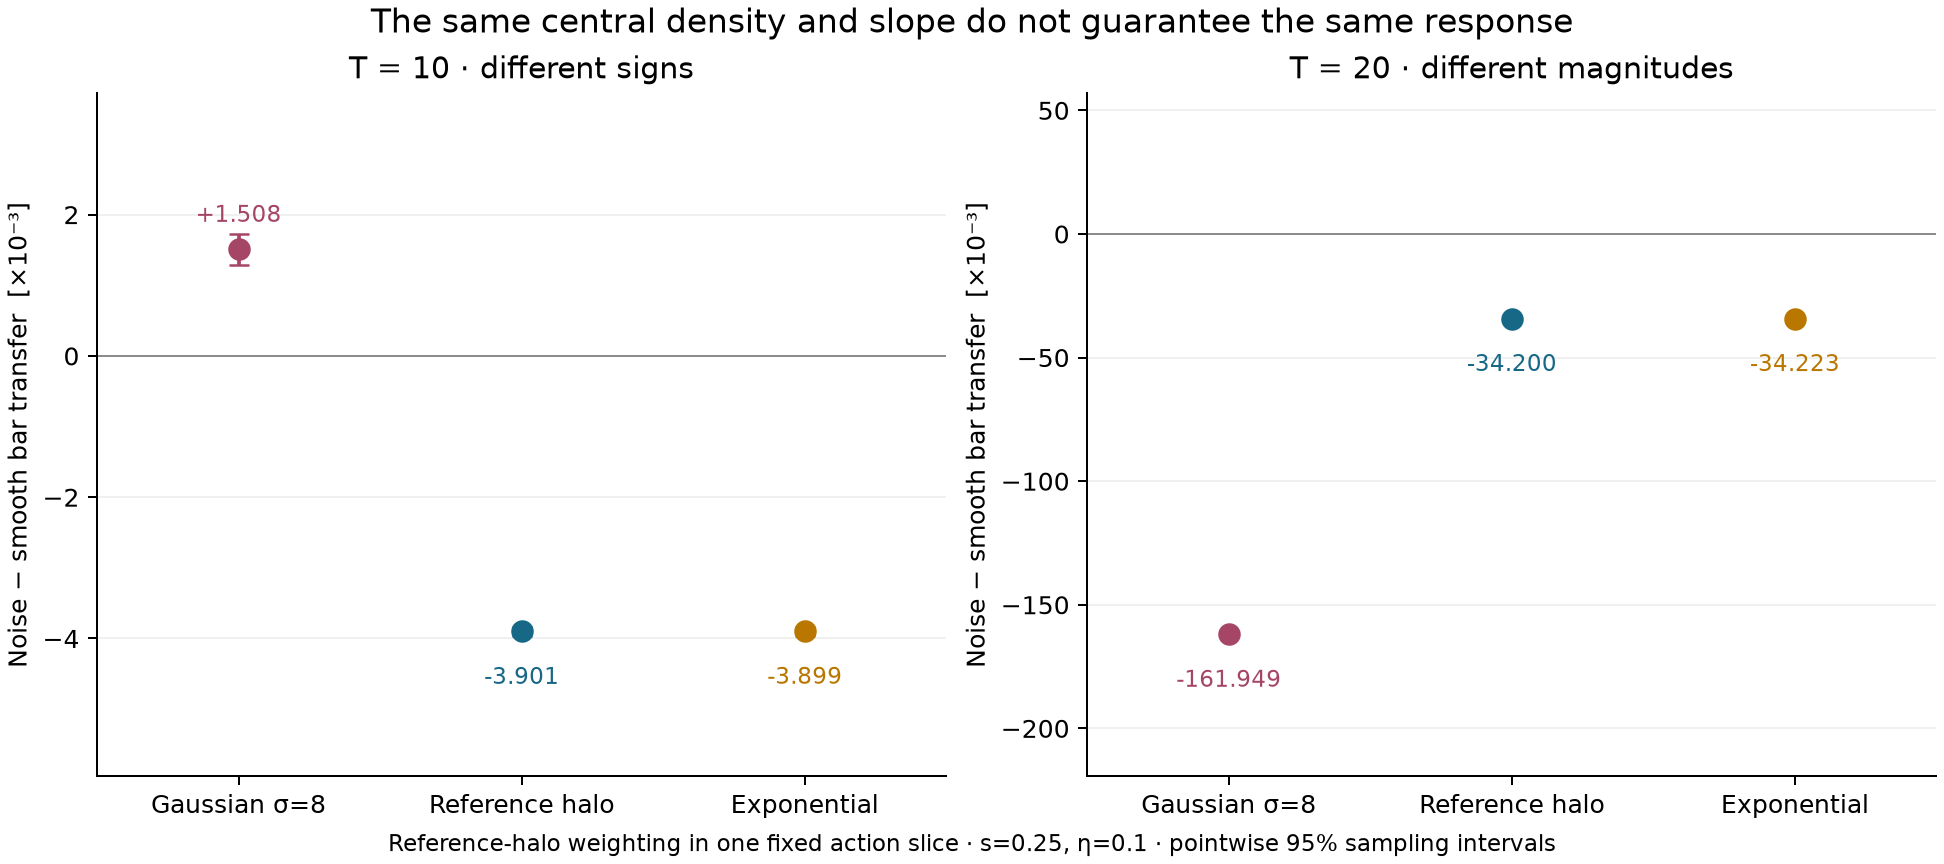
\includegraphics[width=\textwidth]{population-comparison.png}
\caption{Change in accumulated bar transfer caused by diffusion, for populations with the same density and slope at the initial resonance. The Gaussian gives the wrong early sign relative to the reference halo weighting and a larger late suppression; the exponential closely follows the reference. Both panels use s = 0.25, \(\eta\) = 0.1 and the cutoff-40 window. The ordinate is the dimensionless response \(\mathcal R[w]\), conditional on one fast-action slice. Error bars are pointwise 95 per cent Student-t intervals from eight independent batches; they do not include numerical sensitivity. The panels show two measured endpoints, with different vertical scales. \href{https://djova.ca/galaxy-bar/results/populations.json}{Values and numerical controls}.}\label{F-POP-01}
\end{figure*}

\begin{table*}
\centering
\caption{Original population comparison (F-POP-01). Dimensionless noise-minus-smooth accumulated transfer at $s=0.25$, $\eta=0.1$ and cutoff 40. Pointwise 95 per cent intervals use eight independent batches. All six rows pass the declared numerical/window checks. Central density is fixed; weights are not normalized to unit mass.}\label{tab-pop}
\small
\setlength{\tabcolsep}{4pt}
\begin{tabular}{lrrrr}
\toprule
Population & $T$ & $\mathcal R$ & 95 per cent lower & 95 per cent upper \\
\midrule
Gaussian $\sigma=8$ & 10 & 0.00150764622 & 0.00128939881 & 0.00172589363 \\
Halo & 10 & -0.00390067586 & -0.00396285817 & -0.00383849356 \\
Exponential & 10 & -0.0038987336 & -0.00396095025 & -0.00383651696 \\
Gaussian $\sigma=8$ & 20 & -0.161949145 & -0.162575063 & -0.161323226 \\
Halo & 20 & -0.0342002314 & -0.034326595 & -0.0340738678 \\
Exponential & 20 & -0.0342234835 & -0.0343499518 & -0.0340970151 \\
\bottomrule
\end{tabular}
\end{table*}

This result suggests a more precise question than whether the initial curvature is small. Over which actions must the approximation preserve the population gradient? A difference far from the dynamically relevant region need not affect the transfer. Conversely, a modest difference can matter if it changes the balance of large, oppositely signed contributions. We use the response kernel to identify that region and measure this balance.

\section{The action-dependent response}\label{kernel}

Because the bar and the noise do not depend on the population, the orbit calculation can be performed before choosing its weight. Define

\begin{equation}\label{EQ-KER-01}
\begin{aligned}
K_B(x)&=\mathbb E[B_{\rm noise}-B_{\rm smooth}\mid x],\\
\mathcal R[w]&=\int w(x)K_B(x)\,\mathrm dx.
\end{aligned}
\end{equation}

The expectation averages over initial phase and noise. The kernel measures what the imposed dynamics do to particles starting at \(x\); the weight specifies how much material starts there. Trapping can make an individual trajectory highly nonlinear without spoiling this separation. It requires only that changing the population leave the evolution law unchanged.

Let \(Q_{\rm p}\) be a primitive of \(K_B\). Integration by parts gives

\begin{equation}\label{EQ-GRAD-01}
\mathcal R[w]=[wQ_{\rm p}]_{\rm boundary}
-\int w'(x)Q_{\rm p}(x)\,\mathrm dx.
\end{equation}

Figure \ref{F-GRAD-01} displays the ingredients of this integral. The boundary term vanishes for the compact windows used here. This form shows exactly which population gradients matter: the contribution at each action is \(-w'Q_{\rm p}\). It also explains why agreement at the initial resonance is insufficient. The Gaussian changes the derivative away from that point, where the primitive kernel can still be appreciable.

\begin{figure*}
\centering
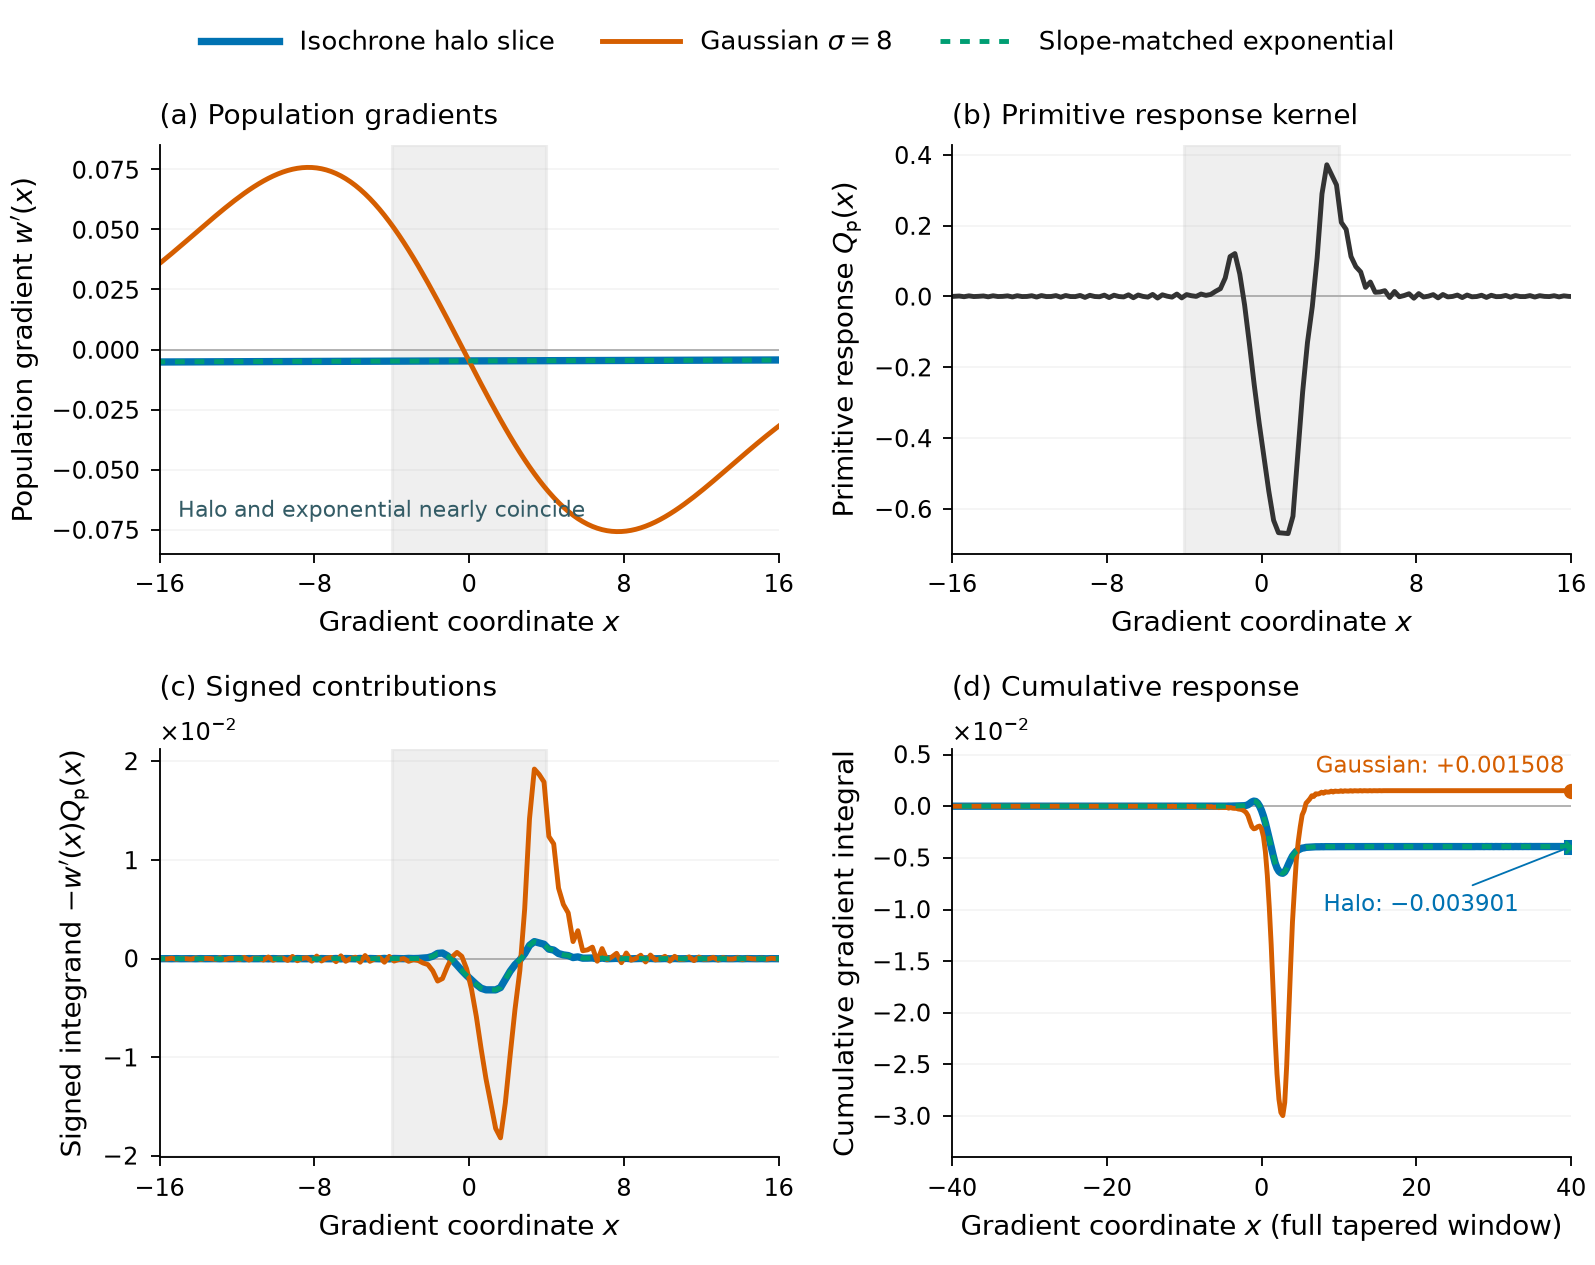
\includegraphics[width=\textwidth]{population-gradient-explanation.png}
\caption{How population gradients weight the recorded response at T = 10, s = 0.25 and \(\eta\) = 0.1. (a) Population gradients; (b) their common primitive kernel; (c) signed contributions to the gradient integral; (d) cumulative response across the complete cutoff-40 window. The grey strip marks \(|x|<4\). Panels (a)--(c) show the central interval \(|x|\leq16\). Products are evaluated on the original fine cells before summation into display cells; multiplying the displayed mean curves is not equivalent. Shaded curve bands are pointwise 95 per cent Student-t intervals from eight batches, without numerical-error expansion. These are terms in the integration-by-parts representation, not separate cohorts of initial orbits. The explanatory curves describe the recorded kernel estimate; the sampling and numerical checks for the endpoint values are supplied with Figure \ref{F-POP-01}.}\label{F-GRAD-01}
\end{figure*}

For the Gaussian at \(T=10\), integrating the gradient contribution inside and outside \(|x|=4\) gives approximately \(-0.011058\) and \(+0.012565\). Their sum is positive. For the halo, the corresponding contributions are \(-0.004835\) and \(+0.000934\), giving a negative sum. The Gaussian's imposed curvature changes this balance enough to reverse the sign. The exponential, whose gradient remains close to the halo's over the relevant interval, largely preserves it.

This decomposition explains the population dependence of the measured response. It does not by itself separate diffusion-supported friction from changes in resonant capture: that would require additional dynamical diagnostics. Its use here is to calculate several population responses from one set of trajectories and to make the error of a chosen approximation explicit.

\section{Testing a population approximation}\label{accuracy}

Suppose \(h\) is the reference weight and \(v\) an approximation. Subtracting their gradient representations gives a signed integral of \(v'-h'\). Taking its absolute value yields

\begin{equation}\label{EQ-ERR-01}
\left|\mathcal R[v]-\mathcal R[h]\right|
\leq \int |v'(x)-h'(x)|\,|Q_{\rm p}(x)|\,\mathrm dx.
\end{equation}

This bound is exact for an exact kernel and the stated boundary treatment. It is small when the approximation preserves the gradient where the response is sensitive. Its limitation is equally clear: taking absolute values loses cancellations, so the bound can be larger than the actual error.

In practice, \(Q_{\rm p}\) is estimated from trajectories. We enlarge the gradient integral to account for its sampling uncertainty and measured numerical sensitivity, then add the uncertainty in the approximate response itself. We accept an approximation at the requested accuracy only when this total allowance lies below the target. For the 5 per cent tests, the absolute target is set using a conservative lower estimate of the reference response. A separate sign test asks whether the expanded response interval excludes zero.

The sampling calculation uses eight independent batches and a Student-t envelope with Bonferroni allocation over the specified kernel cells and scalar estimates. Paired timestep differences and factor-two mesh refinements supply numerical-error estimates. These choices produce a reproducible decision rule, but its coverage is approximate: the exact inequality does not turn sampled kernels or refinement differences into rigorous error bounds.

We tested the rule at \(s=0.5\), twice the original sweep rate, keeping \(\eta=0.1\). The new dynamics require a new kernel. The candidate family comprises the exponential and Gaussians with \(\sigma=8,32,128,512\), at both endpoints and both windows. These choices and the decisions were fixed before the independent distribution calculations were examined. Figure \ref{F-ACC-01} compares the resulting error allowances with the independent outcomes. Among twenty candidate comparisons, the rule accepted eight: the exponential and Gaussian of width 512 at two times and two windows. All eight meet the specified 5 per cent target in the independent calculation, including its numerical-error estimates. The comparisons share one dynamical condition and one sampled kernel; their count does not represent eight independent physical regimes.

\begin{figure*}
\centering
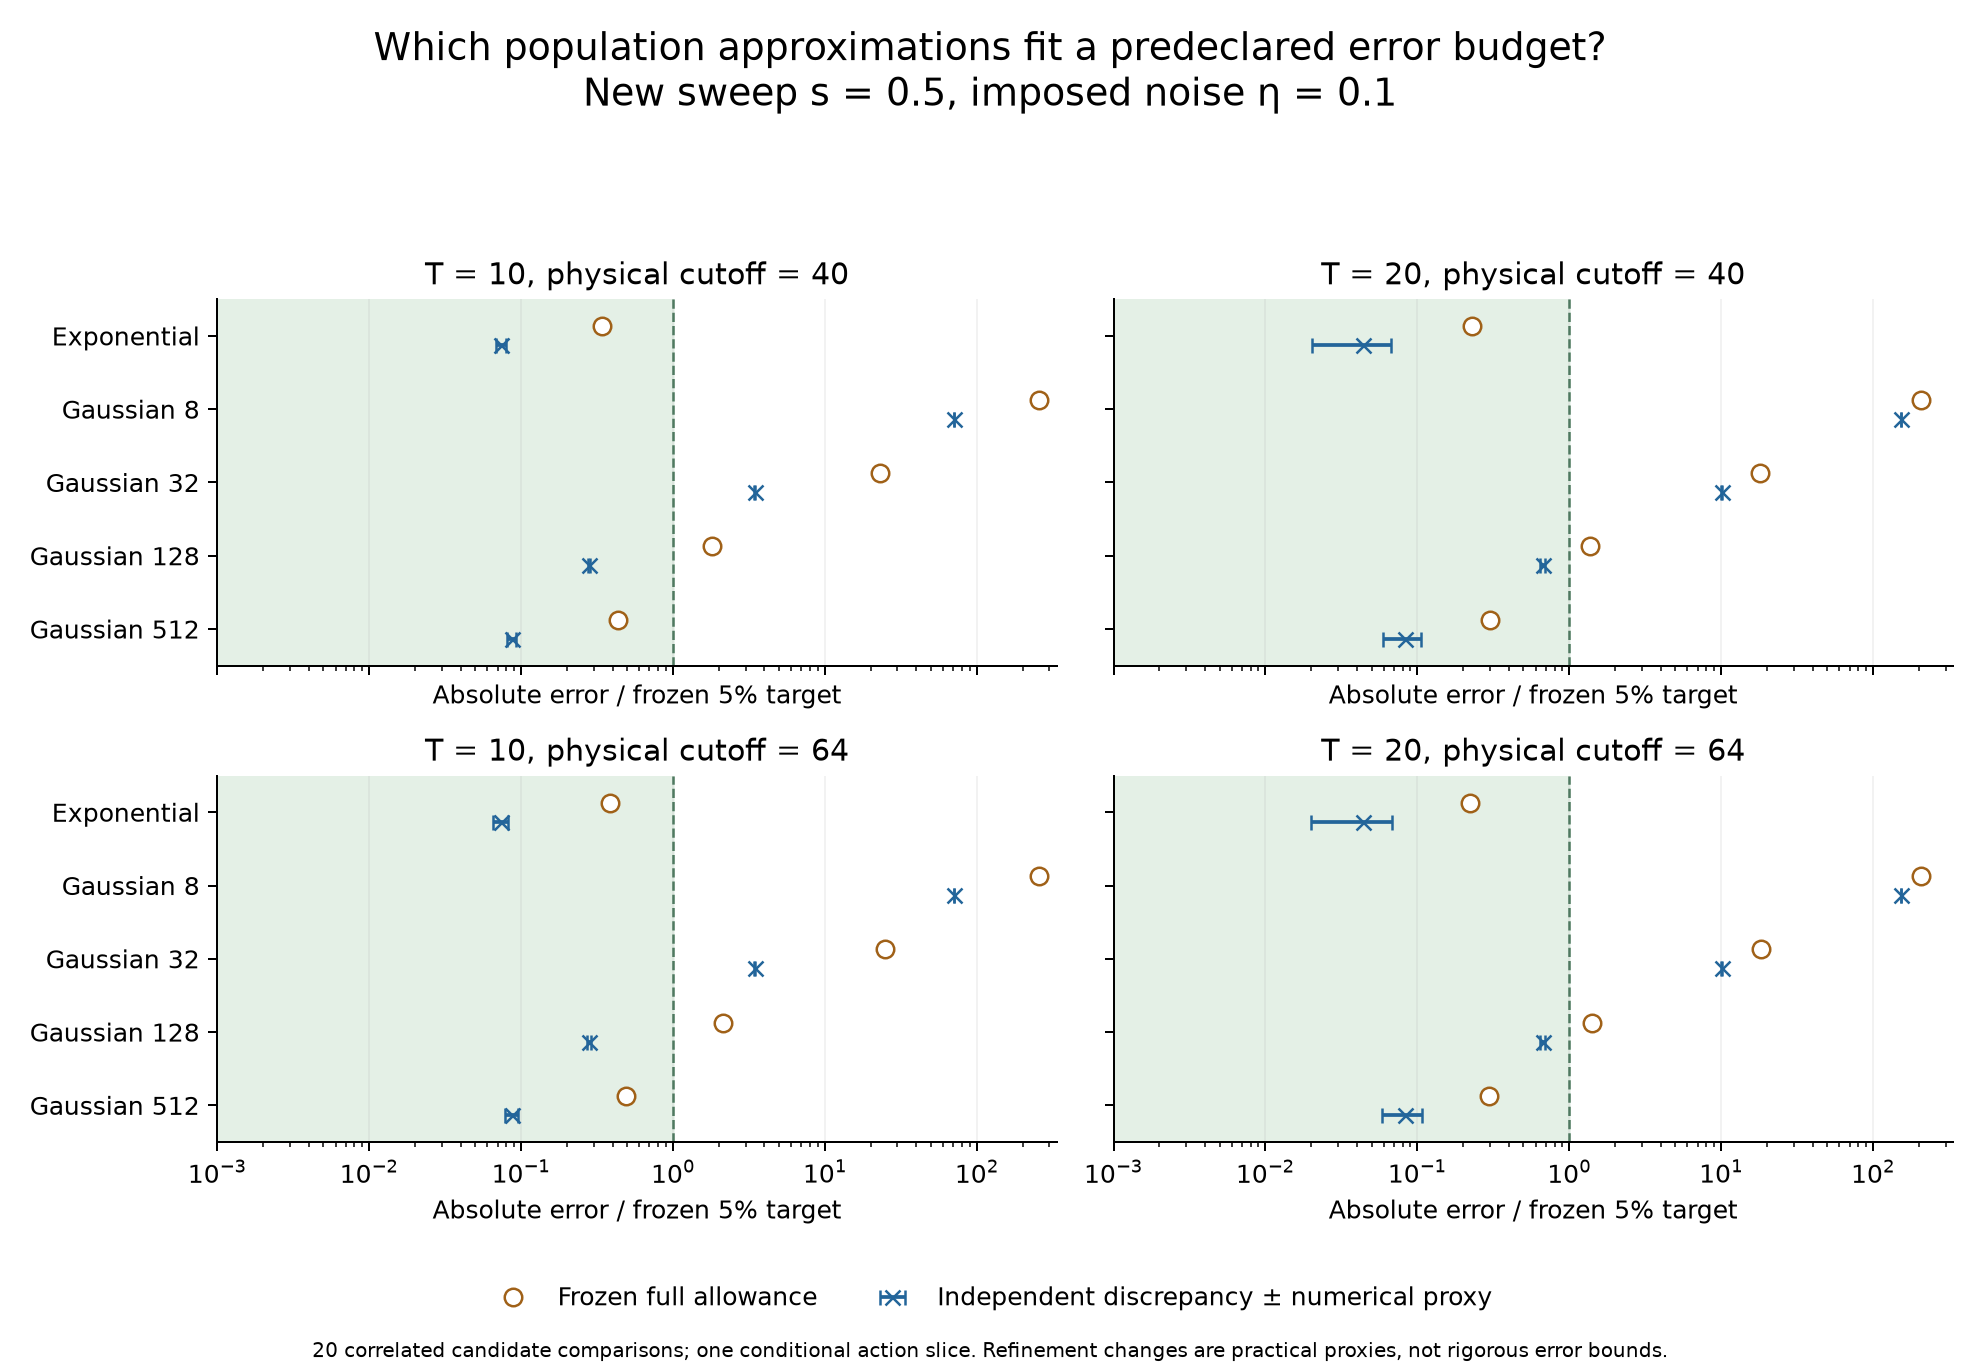
\includegraphics[width=\textwidth]{population-accuracy.png}
\caption{Performance of the population-error test at s = 0.5 and \(\eta\) = 0.1. Orange circles show the total error allowance divided by the frozen 5 per cent target. Blue crosses show the discrepancy between the approximate response predicted from the kernel and the independently evolved halo response, expanded by the halo's numerical-error estimate and divided by the same target. The latter includes kernel-estimation error, whereas the intrinsic population error compares independently evolved populations. All eight accepted candidates meet the target. Four Gaussian-128 comparisons also meet it but are rejected by the test; eight remaining candidates are independently outside the target. Four halo self-references are excluded from these counts. \href{https://djova.ca/galaxy-bar/paper.html\#table-accuracy}{Full values}.}\label{F-ACC-01}
\end{figure*}

The four conservative rejections illustrate the cost of discarding cancellation. For Gaussian 128 at \(T=10\) in the primary window, the signed population contrast from the mean kernel is approximately \(9.48\times10^{-5}\) in magnitude. The integral of the absolute gradient contributions is \(5.20\times10^{-4}\), already larger than the \(4.38\times10^{-4}\) target before adding kernel uncertainty. More precise kernel sampling does not restore the cancellation discarded by taking absolute values. The test can therefore identify useful approximations while declining some that would in fact be accurate.

Complete values are in Appendix \ref{app-accuracy}; the interactive article provides the downloadable unrounded records.

Computing the new kernel required about 5,105 worker CPU-seconds; evaluating the six-profile diagnostic took about 0.8 seconds. The kernel is the expensive step. Once it and the full reference DF are available, directly contracting them is also cheap. The error test is useful for assessing a simplifying population choice, not as a claim that approximating a known DF is always faster than using it.

\section{Estimating small transfers efficiently}\label{estimator}

Directly averaging weighted impulses can be inefficient. An individual orbit may gain or lose much more angular momentum than the net transfer of a broad population. The estimate then depends on cancellation between large sampled terms. We reduce that variance by subtracting a control whose integrated expectation is known to vanish.

Let \(F'=w\). From the action budget, removing the coordinate shift and random impulse gives \(y=j+sT-\Xi_T=x+B\). For a fixed noise history, the map from the initial phase plane to \(\psi,y\) preserves area. The time derivative of the integrated primitive displacement can therefore be written as an integral of \(-w(y)\sin\psi\) over that plane. Its angular average vanishes, and the primitive displacement is initially zero. With uniform initial phase and sufficient auxiliary action support, the finite displacement \(F(x+B)-F(x)\) has zero integrated expectation. Consequently,

\begin{equation}\label{EQ-EST-01}
\begin{aligned}
\int w(x)\,\mathbb E[B]\,\mathrm dx
&=-\int\mathbb E\!\left[R_w(x,B)\right]\,\mathrm dx,\\
R_w(x,B)&=F(x+B)-F(x)-w(x)B.
\end{aligned}
\end{equation}

The left-hand side is the generally nonzero transfer. On the right, the first-order term has cancelled \emph{inside the remainder}. For a weight that varies slowly over the displacement, the remainder begins with \(w'B^2/2\); the estimator uses its negative. This replaces a large fluctuating impulse by a smaller quantity controlled by the variation of the weight.

The identity needs more than area preservation alone. The auxiliary initial-action region must extend beyond the physical support by the maximum bar impulse, so that translated trajectories are accounted for even when their starting weights vanish. Those auxiliary samples add no physical mass. The \href{https://djova.ca/galaxy-bar/methods/CUMULATIVE_IDENTITY.md}{derivation} specifies the support and symmetry assumptions; action-dependent noise, nonuniform initial phases or a responding halo require a new argument. We apply the identity separately to the noisy and smooth transfers and subtract them.

Variance reduction by subtracting a known contribution is established practice. In cosmological neutrino calculations, \citet{Elbers2021} use a \(\delta f\) construction to sample departures from a reference distribution. Our control instead uses the finite-displacement identity for the accumulated bar impulse. The useful question is how much this particular construction reduces variance for the present target, and where it ceases to help.

\begin{figure*}
\centering
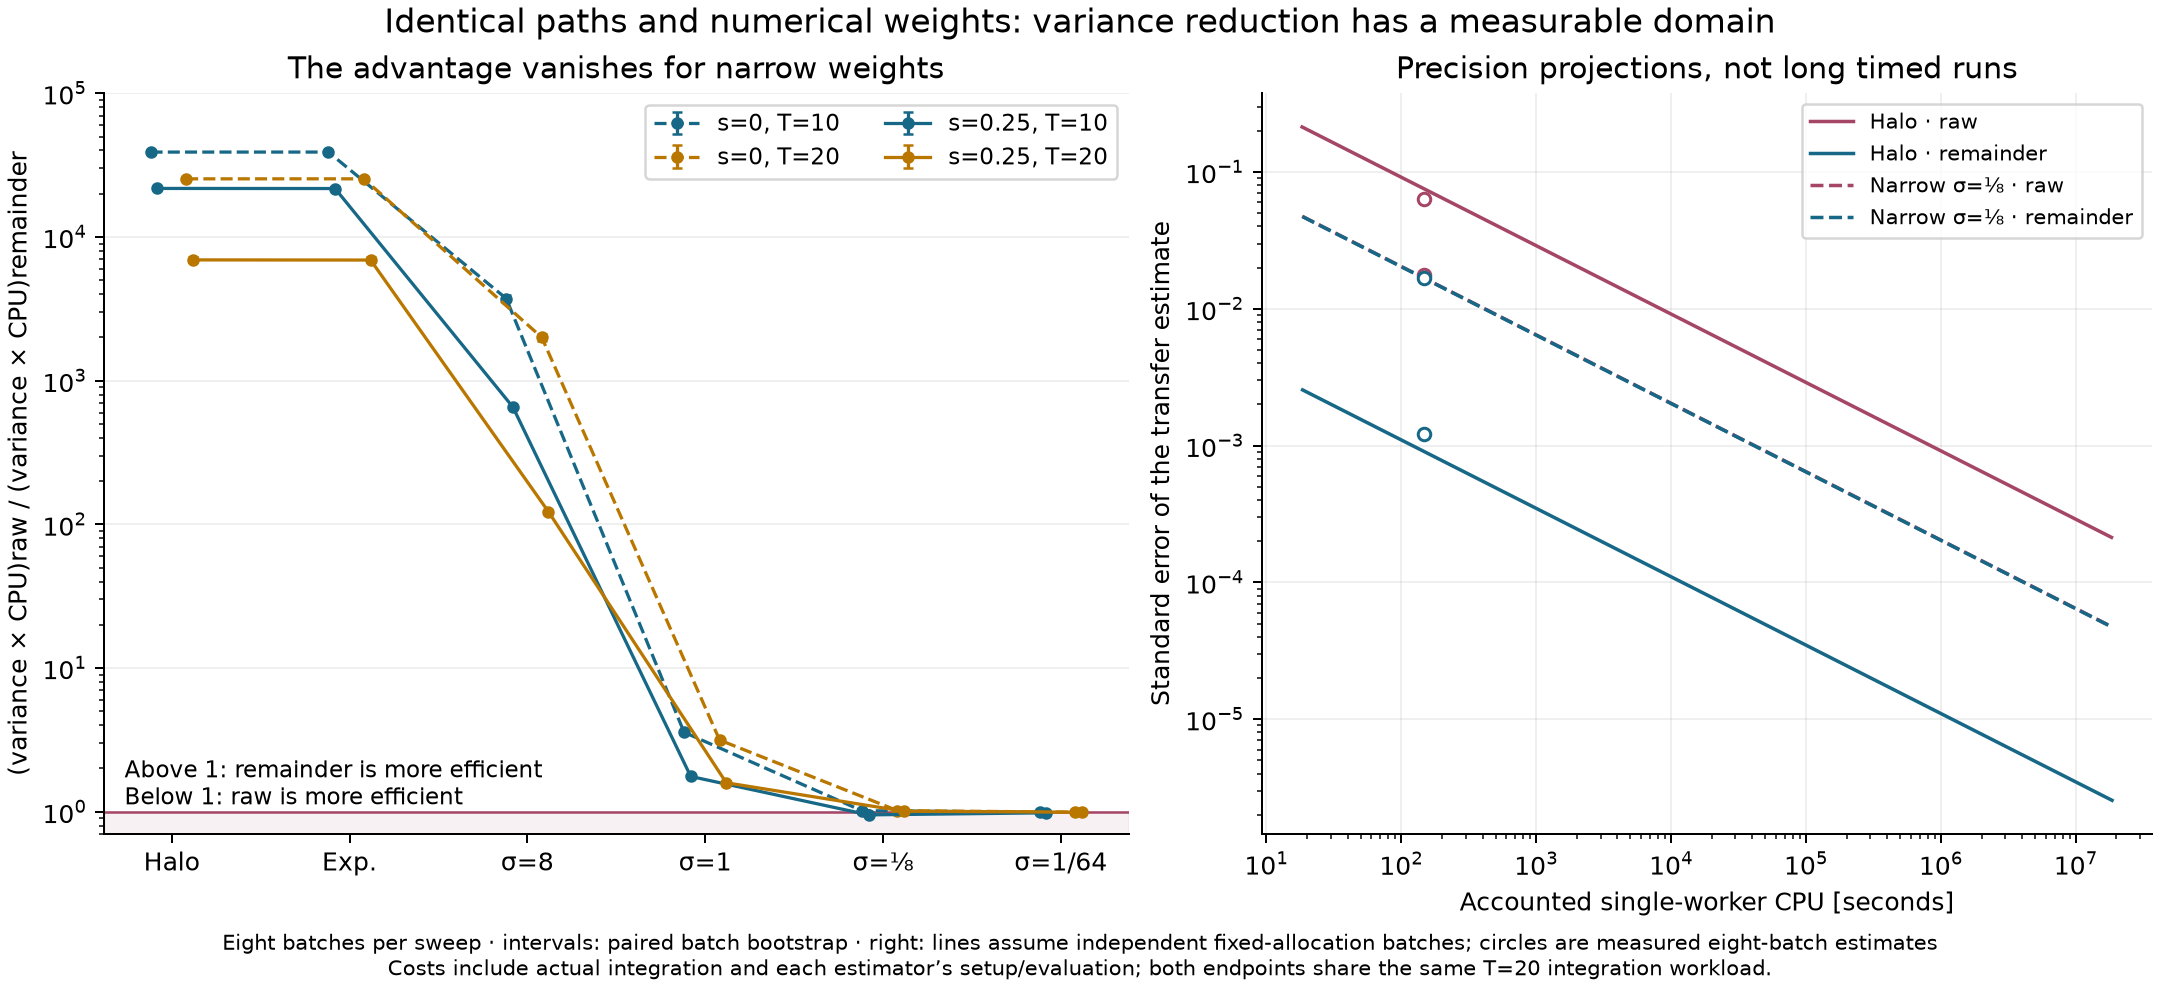
\includegraphics[width=\textwidth]{estimator-efficiency.png}
\caption{Efficiency of the finite-displacement estimator on matched paths and weights. Left: raw-to-remainder cost-times-variance ratio. Right: precision projected under independent repetition of the measured batch workload, with circles marking the eight-batch estimates. The broad halo population benefits strongly, whereas the narrowest Gaussian does not. Costs include trajectory integration to T = 20, paired timestep refinement, setup and method-specific evaluation; both methods exclude I/O and common covariance assembly. T = 10 receives the same full-workload cost. Intervals are whole-batch bootstrap intervals. Conditional and between-batch variance estimates are reported separately in the \href{https://djova.ca/galaxy-bar/paper.html\#table-cost}{complete records}.}\label{F-COST-01}
\end{figure*}

Figure \ref{F-COST-01} shows the measured efficiency across broad and narrow weights. For the halo weight at \(s=0.25\), \(T=20\), the raw and remainder calculations cost about 18.40 and 18.56 CPU-seconds per batch. Their conditional cost-times-variance ratio is approximately 6,928; using the noisier variance between the eight batches gives about 2,749. The gain comes from lower variance, not faster orbit integration. For a Gaussian of width \(1/64\), the ratio is about 0.993 and the advantage disappears, as expected when the weight changes sharply over an impulse displacement. One of the 24 pointwise paired method-comparison intervals excludes zero; it remains in the record and is not, by itself, evidence of bias after multiple comparisons.

Complete values are in Appendix \ref{app-cost}, with paired intervals for every recorded endpoint.

\section{Discussion and conclusions}\label{limitations}

The population choice can alter a finite-time noise response even when central density and slope are matched. In our example, the Gaussian gives the opposite early sign from the reference halo slice and a late suppression about 4.7 times larger. The exponential succeeds much better because its gradient follows the reference over the actions that contribute to the response. The relevant matching condition is therefore distributed over that interval, rather than confined to the initial resonance.

The response kernel makes this statement quantitative. It identifies how changes in the population gradient affect the transfer and provides an error test that can be evaluated before a new population is evolved. At the second sweep rate, the accepted approximations satisfy the independent numerical comparison. The conservative rejections show that this usefulness comes with a limitation: an absolute bound can discard cancellation essential to the final answer. A failure to accept an approximation need not mean that the approximation is inaccurate.

These conclusions concern a fixed external evolution. The halo DF enters as an initial weight on one pair of fast actions; it does not generate a responding potential. In a self-consistent system, redistribution of particles can alter the forces and resonance locations. The connection between DF structure and dynamical friction in such systems is discussed, for example, by \citet{Dattathri2026}, but their collective core dynamics are absent from this model. The present calculation neither measures a full-halo torque nor provides a universal correction for one.

The constant coefficients, additive diffusion, finite population window and abrupt bar turn-on further define the scope of the result. A different history or noise law requires a new kernel. Our attempted transfer to prescribed-field three-dimensional orbits remains statistically unresolved; even successful agreement there would leave collective halo response untested. The noise coefficient has not been calibrated to dark-matter scattering. \textbf{These experiments do not test CDM against SIDM.}

\protect\phantomsection\label{conclusions}{} The practical result is a way to assess a population substitution in a controlled resonance calculation: compare its gradient with the reference over the region weighted by the kernel, retain cancellation when computing the response, and include kernel uncertainty when assessing the error. The finite-displacement estimator makes that assessment affordable for broad populations. Its extension to a broader range of resonances and noise histories can be tested independently of the population example presented here.

\section*{Acknowledgements and disclosure}
This manuscript typesets the existing Galaxy Bar interactive publication \citep{GalaxyBar2026}. The human project maintainer is djova; analysis, software and exposition were developed with AI assistance. No institutional affiliation, independent scientific review or journal endorsement is asserted. The MNRAS class and BibTeX style are supplied by the Royal Astronomical Society under the LaTeX Project Public License.
\section*{Data availability}
The article, protocols, numerical records and executable benchmark are public at \url{https://github.com/djova/bar-halo-benchmark}. The interactive article is \url{https://djova.ca/galaxy-bar/paper.html}. Scientific evidence is pinned by publication release 2026-09-24.2. This PDF is export 2026-09-24.3; it does not report a new simulation. Complete derivations and data definitions are linked from the article. The benchmark's MIT licence applies as recorded there; third-party works retain their own terms.
\bibliographystyle{mnras}
\bibliography{references}
\clearpage
\onecolumn
\makeatletter
\def\fps@table{!h}
\makeatother
\appendix
\renewcommand{\theHtable}{\thesection.\arabic{table}}
\section{Complete accuracy records}\label{app-accuracy}

The earlier population-forecast study used a different rule, the larger of 0.0002 and 5 per cent of the forecast. Its 24 original passes remain recorded; two early Gaussian-12 comparisons remain marginal when later numerical-error estimates are combined. They are not part of the new-condition accuracy test below. The interactive evidence appendix retains their complete assessment.

At \(s=0.5\) and \(\eta=0.1\), Q/NQ denotes the advance qualification; in/out denotes whether the independent comparison supports accuracy within 5 per cent or lies outside it. The 24 rows contain twenty candidates and four halo references; they share one dynamical condition. Tables report rounded values; the public JSON/CSV retains full precision.

\begin{table}
\centering
\caption{Prospective operational decisions (PA-ACC-01, PA-ACC-02). $c$ is the physical window cutoff, $\widehat{\mathcal R}$ the kernel forecast, $\mathcal R_{\rm ind}[v]$ independent evolution of the indicated population, $A$ the full allowance and $\epsilon$ the frozen absolute 5 per cent target. The in/out assessment compares the forecast with the independently evolved halo, with the supplied numerical proxy; it is not a general confidence guarantee.}\label{tab-acc}
\small
\setlength{\tabcolsep}{4pt}
\begin{tabular}{lrrrrrrl}
\toprule
Population & $T$ & $c$ & $\widehat{\mathcal R}$ & $\mathcal R_{\rm ind}[v]$ & $A$ & $\epsilon$ & Decision \\
\midrule
Halo (ref.) & 10 & 40 & -0.00886739 & -0.00884001 & 0.000113244 & 0.000437707 & Q/in \\
Exponential & 10 & 40 & -0.00887235 & -0.00884492 & 0.000148862 & 0.000437707 & Q/in \\
Gaussian 8 & 10 & 40 & -0.0398136 & -0.039611 & 0.113124 & 0.000437707 & NQ/out \\
Gaussian 32 & 10 & 40 & -0.0103457 & -0.0103051 & 0.0100395 & 0.000437707 & NQ/out \\
Gaussian 128 & 10 & 40 & -0.00896218 & -0.00893389 & 0.000794601 & 0.000437707 & NQ/in \\
Gaussian 512 & 10 & 40 & -0.00887795 & -0.00885047 & 0.000189338 & 0.000437707 & Q/in \\
Halo (ref.) & 10 & 64 & -0.00886971 & -0.00884243 & 0.000125126 & 0.000437229 & Q/in \\
Exponential & 10 & 64 & -0.00887466 & -0.00884733 & 0.000167582 & 0.000437229 & Q/in \\
Gaussian 8 & 10 & 64 & -0.0398136 & -0.039611 & 0.112054 & 0.000437229 & NQ/out \\
Gaussian 32 & 10 & 64 & -0.0103469 & -0.0103062 & 0.0108583 & 0.000437229 & NQ/out \\
Gaussian 128 & 10 & 64 & -0.00896442 & -0.00893618 & 0.000929585 & 0.000437229 & NQ/in \\
Gaussian 512 & 10 & 64 & -0.00888026 & -0.00885287 & 0.000215717 & 0.000437229 & Q/in \\
Halo (ref.) & 20 & 40 & -0.0661634 & -0.0661332 & 0.000546073 & 0.00328087 & Q/in \\
Exponential & 20 & 40 & -0.0662763 & -0.0662461 & 0.000753038 & 0.00328087 & Q/in \\
Gaussian 8 & 20 & 40 & -0.570825 & -0.570686 & 0.675507 & 0.00328087 & NQ/out \\
Gaussian 32 & 20 & 40 & -0.0991752 & -0.0991428 & 0.0593474 & 0.00328087 & NQ/out \\
Gaussian 128 & 20 & 40 & -0.0683291 & -0.0682987 & 0.00451777 & 0.00328087 & NQ/in \\
Gaussian 512 & 20 & 40 & -0.0664046 & -0.0663743 & 0.000988743 & 0.00328087 & Q/in \\
Halo (ref.) & 20 & 64 & -0.0661736 & -0.0661429 & 0.000519889 & 0.00328269 & Q/in \\
Exponential & 20 & 64 & -0.0662865 & -0.0662558 & 0.000733738 & 0.00328269 & Q/in \\
Gaussian 8 & 20 & 64 & -0.570825 & -0.570686 & 0.674266 & 0.00328269 & NQ/out \\
Gaussian 32 & 20 & 64 & -0.0991807 & -0.0991478 & 0.0601307 & 0.00328269 & NQ/out \\
Gaussian 128 & 20 & 64 & -0.0683388 & -0.068308 & 0.00461589 & 0.00328269 & NQ/in \\
Gaussian 512 & 20 & 64 & -0.0664147 & -0.066384 & 0.000977177 & 0.00328269 & Q/in \\
\bottomrule
\end{tabular}
\end{table}

\begin{table}
\centering
\caption{Independent intrinsic population error and forecast discrepancy. $e=\mathcal R_{\rm ind}[v]-\mathcal R_{\rm ind}[h]$; $p_e$ is its numerical-refinement proxy; $\delta=\widehat{\mathcal R}[v]-\mathcal R_{\rm ind}[h]$; $p_h$ is the halo proxy. All quantities are dimensionless accumulated response differences. Proxies are not sampling intervals or proved bounds.}\label{tab-errors}
\small
\setlength{\tabcolsep}{4pt}
\begin{tabular}{lrrrrrr}
\toprule
Population & $T$ & $c$ & $e$ & $p_e$ & $\delta$ & $p_h$ \\
\midrule
Halo & 10 & 40 & 0 & 0 & -2.73791e-05 & 2.34302e-06 \\
Exponential & 10 & 40 & -4.91079e-06 & 7.70468e-09 & -3.23376e-05 & 2.34302e-06 \\
Gaussian 8 & 10 & 40 & -0.030771 & 3.05131e-05 & -0.0309736 & 2.34302e-06 \\
Gaussian 32 & 10 & 40 & -0.00146509 & 2.23114e-06 & -0.00150574 & 2.34302e-06 \\
Gaussian 128 & 10 & 40 & -9.38843e-05 & 1.47467e-07 & -0.000122174 & 2.34302e-06 \\
Gaussian 512 & 10 & 40 & -1.04625e-05 & 1.64426e-08 & -3.79434e-05 & 2.34302e-06 \\
Halo & 10 & 64 & 0 & 0 & -2.72805e-05 & 3.59106e-06 \\
Exponential & 10 & 64 & -4.90328e-06 & 1.07603e-08 & -3.22344e-05 & 3.59106e-06 \\
Gaussian 8 & 10 & 64 & -0.0307685 & 2.96698e-05 & -0.0309711 & 3.59106e-06 \\
Gaussian 32 & 10 & 64 & -0.00146374 & 2.43893e-06 & -0.00150452 & 3.59106e-06 \\
Gaussian 128 & 10 & 64 & -9.37495e-05 & 1.95532e-07 & -0.000121991 & 3.59106e-06 \\
Gaussian 512 & 10 & 64 & -1.04468e-05 & 2.24912e-08 & -3.78352e-05 & 3.59106e-06 \\
Halo & 20 & 40 & 0 & 0 & -3.0203e-05 & 7.69542e-05 \\
Exponential & 20 & 40 & -0.000112873 & 3.18237e-07 & -0.000143083 & 7.69542e-05 \\
Gaussian 8 & 20 & 40 & -0.504552 & 0.000928533 & -0.504691 & 7.69542e-05 \\
Gaussian 32 & 20 & 40 & -0.0330096 & 9.04521e-05 & -0.033042 & 7.69542e-05 \\
Gaussian 128 & 20 & 40 & -0.00216553 & 6.11218e-06 & -0.00219586 & 7.69542e-05 \\
Gaussian 512 & 20 & 40 & -0.000241147 & 6.80996e-07 & -0.000271365 & 7.69542e-05 \\
Halo & 20 & 64 & 0 & 0 & -3.07105e-05 & 7.85303e-05 \\
Exponential & 20 & 64 & -0.000112849 & 3.14117e-07 & -0.000143568 & 7.85303e-05 \\
Gaussian 8 & 20 & 64 & -0.504543 & 0.00092746 & -0.504682 & 7.85303e-05 \\
Gaussian 32 & 20 & 64 & -0.0330049 & 8.97729e-05 & -0.0330378 & 7.85303e-05 \\
Gaussian 128 & 20 & 64 & -0.00216509 & 6.04033e-06 & -0.00219594 & 7.85303e-05 \\
Gaussian 512 & 20 & 64 & -0.000241097 & 6.72499e-07 & -0.000271824 & 7.85303e-05 \\
\bottomrule
\end{tabular}
\end{table}

\clearpage
\section{Complete matched estimator records}\label{app-cost}

These are cost-times-variance ratios under the specified matched workload, not direct simulation speedups. All 24 endpoints retain their numerical values and paired method-consistency intervals. Gaussian stress labels give the width \(\sigma\).

\begin{table}
\centering
\caption{Matched estimator costs and variance ratios (EST-01). $C_{\rm raw}$ and $C_{\rm rem}$ are mean CPU seconds per accounted batch; $V_C$ is the conditional raw/remainder cost-times-variance ratio; brackets give its whole-batch bootstrap interval; $V_B$ uses between-batch variance. All $T=10$ endpoints carry the same full $T=20$ workload cost.}\label{tab-cost}
\small
\setlength{\tabcolsep}{4pt}
\begin{tabular}{lrrrrrlr}
\toprule
Population & $s$ & $T$ & $C_{\rm raw}$ & $C_{\rm rem}$ & $V_C$ & Bootstrap interval & $V_B$ \\
\midrule
Halo & 0.0 & 10 & 18.293 & 18.464 & 38988.6 & [38009, 40044] & 89013.1 \\
Exponential & 0.0 & 10 & 18.287 & 18.451 & 39002.9 & [38024, 40063] & 89093.7 \\
Gaussian 8 & 0.0 & 10 & 18.288 & 18.447 & 3730.44 & [3579.9, 3919.3] & 6777.03 \\
Gaussian 1 & 0.0 & 10 & 18.289 & 18.446 & 3.57294 & [3.4604, 3.6932] & 2.10966 \\
Gaussian 1/8 & 0.0 & 10 & 18.289 & 18.453 & 1.01674 & [0.99736, 1.0364] & 0.689487 \\
Gaussian 1/64 & 0.0 & 10 & 18.288 & 18.452 & 0.992355 & [0.9825, 0.99866] & 1.17587 \\
Halo & 0.0 & 20 & 18.293 & 18.464 & 25391.9 & [24625, 26167] & 13958 \\
Exponential & 0.0 & 20 & 18.287 & 18.451 & 25401.5 & [24632, 26180] & 13964.1 \\
Gaussian 8 & 0.0 & 20 & 18.288 & 18.447 & 1999.35 & [1891.7, 2113.3] & 1984.37 \\
Gaussian 1 & 0.0 & 20 & 18.289 & 18.446 & 3.15316 & [3.0812, 3.2257] & 2.33289 \\
Gaussian 1/8 & 0.0 & 20 & 18.289 & 18.453 & 1.01791 & [0.99051, 1.0416] & 1.01849 \\
Gaussian 1/64 & 0.0 & 20 & 18.288 & 18.452 & 0.992679 & [0.98239, 0.99954] & 1.06109 \\
Halo & 0.25 & 10 & 18.395 & 18.556 & 21774.2 & [21232, 22389] & 15771.5 \\
Exponential & 0.25 & 10 & 18.389 & 18.549 & 21737.7 & [21193, 22346] & 15751.2 \\
Gaussian 8 & 0.25 & 10 & 18.39 & 18.554 & 655.057 & [642.44, 668.69] & 595.86 \\
Gaussian 1 & 0.25 & 10 & 18.391 & 18.558 & 1.76013 & [1.7269, 1.7919] & 1.51852 \\
Gaussian 1/8 & 0.25 & 10 & 18.392 & 18.555 & 0.95067 & [0.92971, 0.97081] & 1.21402 \\
Gaussian 1/64 & 0.25 & 10 & 18.391 & 18.556 & 0.982318 & [0.97679, 0.98715] & 1.00221 \\
Halo & 0.25 & 20 & 18.395 & 18.556 & 6928.35 & [6734.7, 7229.1] & 2749.4 \\
Exponential & 0.25 & 20 & 18.389 & 18.549 & 6909.88 & [6719.3, 7205.8] & 2741.03 \\
Gaussian 8 & 0.25 & 20 & 18.39 & 18.554 & 122.402 & [118.57, 126.06] & 48.8071 \\
Gaussian 1 & 0.25 & 20 & 18.391 & 18.558 & 1.59023 & [1.5738, 1.6053] & 1.23894 \\
Gaussian 1/8 & 0.25 & 20 & 18.392 & 18.555 & 1.00717 & [1.0008, 1.0131] & 1.08977 \\
Gaussian 1/64 & 0.25 & 20 & 18.391 & 18.556 & 0.992683 & [0.99099, 0.99423] & 1.04132 \\
\bottomrule
\end{tabular}
\end{table}

\begin{table}
\centering
\caption{Paired raw-minus-remainder method comparison. Intervals are pointwise 95 per cent sampling intervals, not simultaneous tests across all 24 rows. A retained exclusion of zero is a multiple-comparison flag, not by itself proof of estimator bias.}\label{tab-consistency}
\small
\setlength{\tabcolsep}{4pt}
\begin{tabular}{lrrrrrl}
\toprule
Population & $s$ & $T$ & Raw minus remainder & 95 per cent lower & 95 per cent upper & Contains zero \\
\midrule
Halo & 0.0 & 10 & 0.0321698 & -0.0469248 & 0.111264 & yes \\
Exponential & 0.0 & 10 & 0.0321692 & -0.046922 & 0.11126 & yes \\
Gaussian 8 & 0.0 & 10 & 0.032983 & -0.0370078 & 0.102974 & yes \\
Gaussian 1 & 0.0 & 10 & 0.0362236 & 0.00189735 & 0.0705499 & no \\
Gaussian 1/8 & 0.0 & 10 & 0.00903438 & -0.00255065 & 0.0206194 & yes \\
Gaussian 1/64 & 0.0 & 10 & 0.00134259 & -0.000333731 & 0.00301891 & yes \\
Halo & 0.0 & 20 & 0.0559024 & -0.038755 & 0.15056 & yes \\
Exponential & 0.0 & 20 & 0.0558992 & -0.0387521 & 0.150551 & yes \\
Gaussian 8 & 0.0 & 20 & 0.0537144 & -0.030226 & 0.137655 & yes \\
Gaussian 1 & 0.0 & 20 & 0.0316587 & -0.0199932 & 0.0833106 & yes \\
Gaussian 1/8 & 0.0 & 20 & 0.0053972 & -0.0068051 & 0.0175995 & yes \\
Gaussian 1/64 & 0.0 & 20 & 0.000535115 & -0.00124154 & 0.00231177 & yes \\
Halo & 0.25 & 10 & -0.0514801 & -0.154479 & 0.0515188 & yes \\
Exponential & 0.25 & 10 & -0.0514813 & -0.154478 & 0.0515152 & yes \\
Gaussian 8 & 0.25 & 10 & -0.049866 & -0.145109 & 0.0453768 & yes \\
Gaussian 1 & 0.25 & 10 & -0.010653 & -0.043042 & 0.0217359 & yes \\
Gaussian 1/8 & 0.25 & 10 & -0.00136648 & -0.00742977 & 0.00469681 & yes \\
Gaussian 1/64 & 0.25 & 10 & -0.000182043 & -0.00100055 & 0.000636463 & yes \\
Halo & 0.25 & 20 & -0.0525512 & -0.200904 & 0.0958019 & yes \\
Exponential & 0.25 & 20 & -0.0525555 & -0.200907 & 0.0957963 & yes \\
Gaussian 8 & 0.25 & 20 & -0.0567175 & -0.193001 & 0.079566 & yes \\
Gaussian 1 & 0.25 & 20 & -0.0206914 & -0.0522396 & 0.0108569 & yes \\
Gaussian 1/8 & 0.25 & 20 & -0.00043361 & -0.00642131 & 0.00555409 & yes \\
Gaussian 1/64 & 0.25 & 20 & -0.000116105 & -0.0010129 & 0.000780686 & yes \\
\bottomrule
\end{tabular}
\end{table}

\clearpage
\end{document}
